\chapter{Arquitectura e Implementación de la Solución}

\section{Arquitectura}

En este trabajo se propone desarrollar un sistema centralizado capaz de recibir datos de los dispositivos móviles de los conductores y procesarlos para obtener el estado del tráfico en la ciudad de Asunción. La información resultante será enviada en tiempo real a los usuarios para que los mismos puedan elegir trayectos menos congestionados.

La aplicación móvil está pensada inicialmente para dispositivos con sistema operativo Android. La misma, al ser utilizada por el conductor durante su viaje, registrará los datos del trayecto recorrido que servirán para definir el estado de las rutas. Esta aplicación también contará con un mapa de la ciudad de Asunción, que permitirá ver el estado de las carreteras que tengan información suficiente sobre el tráfico en las mismas. 

La aplicación web, se encargará de generar el estado actual de las rutas procesando la información que reciba de los teléfonos de los conductores. Esta información quedará almacenada de forma persistente en el tiempo  y podrá ser utilizada posteriormente con otros fines, ya sean estadísticos o de predicción de tráfico.

\begin{figure}[h]
	\centering
	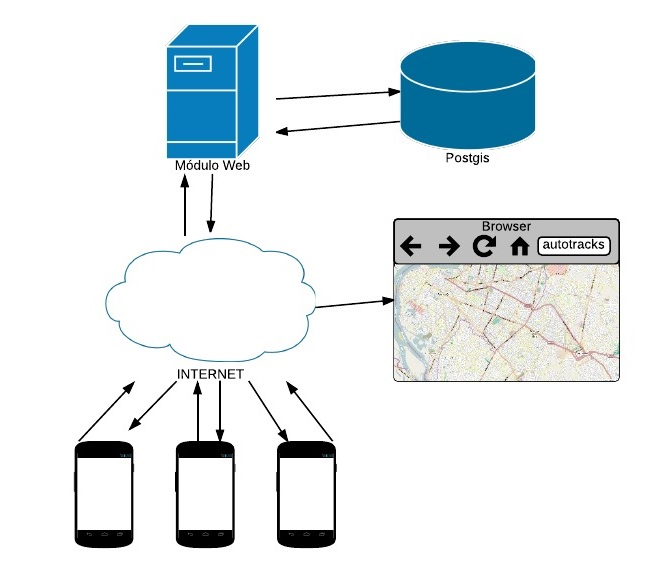
\includegraphics[width=0.7\textwidth]{capitulos/6/figuras/figura1.jpg}
	\caption{\label{fig:arquitectura} Arquitectura del Sistema}	
\end{figure}

Como se puede apreciar en la \Cref{fig:arquitectura}, se tiene un módulo web que consiste en una aplicación web desarrollada en java que corre sobre un servidor de aplicaciones jboss 7. Como motor de base de datos utilizamos postgres en su versión 9.1, el mismo cuenta con la extensión postgis para añadir capacidades GIS y con la extensión pgRouting para las funciones de ruteo geoespacial. Todo esto se encuentra alojado en un servidor privado virtual. Los dispositivos móviles deben contar con el sistema operativo Android en su versión 2.3 (Gingerbread) o superior.

\section{Implementación de la Solución Propuesta}

En esta sección se presentan de manera detallada las herramientas, los datos, los algoritmos y procedimientos utilizados para el sistema de monitoreo de tráfico vehícular Autotracks. Se describen los pasos seguidos para el desarrollo de la aplicación móvil y web.

\subsection{Preparando la Base de Datos}

Para trabajar correctamente con coordenadas se necesita una base de datos Espacial, que a diferencia de las bases de datos relacionales, pueden almacenar y operar sobre datos geométricos. Teniendo como motor de base de datos PostgreSQL, que es relacional, necesitamos añadirle la extensión PostGIS para convertirla en espacial.

Una vez se posea un motor adecuado es necesario obtener la información de los mapas y rutas. A nivel mundial es Google Maps el referente en cuanto a mapas digitales se refiere, pero no permite descargar la información geográfica de los mismos. Por ello optamos por Open Street Maps, un proyecto colaborativo para crear mapas libres y editables, que permite distribuir sus datos bajo licencia abierta Open Database License (ODbL).

Los datos descargados desde Open Street Maps están en el formato OSM XML, que básicamente consiste en una lista de instancias de nodos, caminos y relaciones dentro de su modelo. Para transformar estos datos al formato de Postgis, existe una herramienta llamada osm2pgsql, que es un programa basado en líneas de comando. Como resultado de esta importación se obtienen cuatro tablas:
\begin{enumerate}
\item planet\_osm\_point 
\item planet\_osm\_polygon
\item planet\_osm\_line
\item planet\_osm\_roads
\end{enumerate}
planet\_osm\_point almacena todos los nodos importados, planet\_osm\_polygon almacena todos los polígonos, planet\_osm\_line almacena todas las rutas, y planet\_osm\_roads almacena un subconjunto de las rutas a efectos de renderización a bajos niveles de zoom debido a que planet\_osm\_line contiene demasiados datos para renderizar en estos casos. Estas tablas almacena los datos geométricos con el SRID 900913.

Como también se desean capacidades de enrutamiento, es necesario añadir la extensión pgRouting a PostgreSQL. pgRouting representa toda la información de las rutas como un grafo, siendo los vértices las intersecciones de las calles y las aristas las calles en sí. La longitud de la calle determina su peso, que es utilizado para el cálculo del camino más corto. Para convertir los datos de Open Street Maps se utiliza la herramienta osm2po. Como resultado de esta importación se obtiene una tabla con los datos geométricos almacenados con el SRID 4326.
Para almacenar la información de los usuarios de la aplicación se definieron dos tablas:
\begin{enumerate}
\item localizaciones
\item rutas
\end{enumerate}
en la tabla de localizaciones se guardan los datos de ubicación que son recibidos periódicamente de los usuarios de la aplicación móvil. Se almacena la fecha, la latitud, la longitud, la velocidad, la dirección, la precisión, altitud y la ruta a la que pertenece. Una ruta es un conjunto lógico de localizaciones que es utilizado para el map matching incremental, la ruta representa el recorrido que hace una persona en un viaje.

\subsection{Obteniendo el Floating Car Data}

Para obtener el FCD de los vehículos se desarrolló una aplicación móvil para teléfonos y tabletas con sistema operativo android denominada autotracks (ver \Cref{fig:autotracks}). La misma se encarga de detectar, almacenar y enviar periódicamente las ubicaciones de los usuarios que se estén moviendo de automóviles de manera completamente anónima a un servidor centralizado.

Autotracks tiene tres partes principales en lo que concierne a FCD: 
\begin{itemize}
	\item Detección de Movimiento.
	\item Toma de localizaciones.
	\item Envío de datos al servidor.
\end{itemize}

\begin{figure}[h]
	\centering
	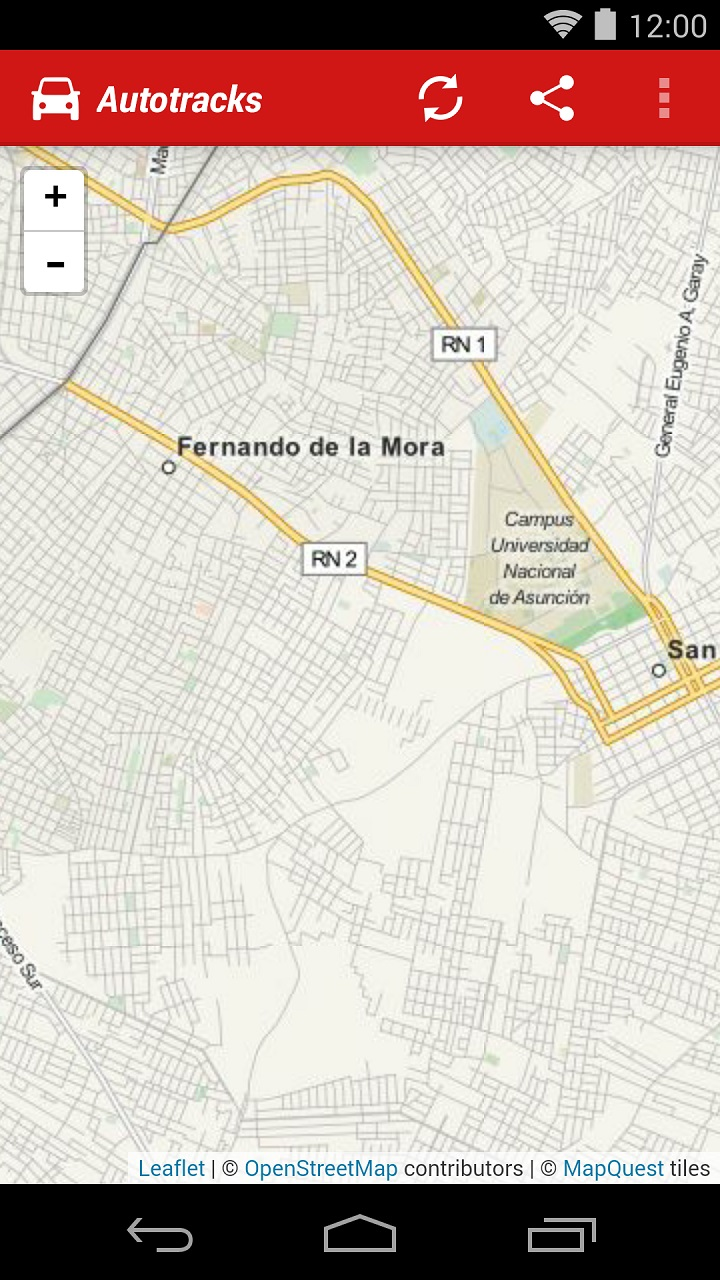
\includegraphics[width=0.5\textwidth]{capitulos/6/figuras/figura2.jpg}
	\caption{\label{fig:autotracks} Vista de Autotracks en un teléfono}	
\end{figure}

\subsubsection{Detección de Movimiento}

Tomar las localizaciones de los usuarios todo el tiempo implicaría un gasto excesivo e innecesario de batería, tomar las localizaciones cuando se tiene abierta la aplicación significaría que el usuario debe iniciar la aplicación manualmente y mantenerla abierta para poder ir registrando su ubicación. Otra alternativa más efectiva es dejar que el usuario inicie y finalice las toma de posiciones, pero nuevamente requiere de la intervención humana.

La forma óptima de registrar las ubicaciones es aquella que no requiera la intervención del usuario y que sea lo suficientemente inteligente para evitar tomar localizaciones no deseadas. Para ello, se necesita una forma de detectar cuando el teléfono se encuentra en movimiento, esto se puede lograr gracias a los sensores con los que cuentan los dispositivos móviles actualmente, especialmente el acelerómetro, que permite medir la aceleración en los ejes coordenados x, y y z de donde se puede estimar la velocidad y el desplazamiento. Una aceleración igual a cero significa que el dispositivo se encuentra quieto, una aceleración mayor a cero implica movimiento.

Incluso la detección no es suficiente para evitar la toma de localizaciones no deseadas como por ejemplo cuando una persona está caminando o andando en bicicleta. Para evitar estos casos es necesario, aparte de detectar el movimiento, reconocer la actividad que se está realizando durante ese movimiento. Existen trabajos como \cite{liao2006location,bao2004activity,ravi2005activity} que permiten detectar la actividad que se está realizando utilizando las posiciones GPS o el acelerómetro del dispositivo.

Específicamente para dispositivos Android existe una solución para el Reconocimiento de Actividad que  viene incluida dentro del Marco de Servicios de Google Play. Este reconocimiento de actividad reconoce cuatro actividades diferentes: quieto, a pie, en bicicleta y en vehículo. Retorna la probabilidad de cada actividad en un momento determinado. Como este framework ya incluye todo lo necesario para la detección de movimiento y actividad, se decidió utilizarlo en Autotracks.

La actividad del usuario es consultada periódicamente con el fin de saber si el mismo se encuentra en un vehículo, en el caso de que así sea se inicia el servicio de toma de ubicaciones y el mismo no se detiene hasta pasados 10 minutos desde la última actividad en vehículo conocida por el usuario, para evitar así que se detenga cuando por ejemplo el vehículo se encuentre quieto a causa de un semáforo. 

\subsubsection{Toma de Localizaciones}

Para obtener la ubicación de los teléfonos inteligentes de hoy en día existen varias opciones posibles, cada una con sus ventajas y desventajas: 
\begin{itemize}
\item \textbf{Triangulación de antenas:} uso mínimo de batería, baja precisión, requiere estar dentro de una red GSM.
\item \textbf{Redes WiFi:} uso bajo de batería, precisión media, es necesario estar en la cercanías de un punto de acceso WiFi, funciona bien en interiores.
\item \textbf{GPS:} uso elevado de batería, alta precisión, no funciona correctamente en interiores.
\end{itemize}
Buscando la mayor flexibilidad posible, se decidió que la aplicación fuera capaz de trabajar con cualquiera de estas opciones para obtener la ubicación de los dispositivos, buscando siempre utilizar la mejor opción disponible. Para ello se utilizó la localización fusionada que se incluye dentro del Marco de Servicios de Google Play.

En los casos en que la localización es obtenida a través de las redes GSM o WiFi no se dispone de la información de velocidad, para paliar esta falta de información, cuando no se puede obtener la velocidad en un punto, la misma es estimada utilizando la ubicación anterior de la siguiente manera
\begin{equation}
v=\frac { d }{ t }
\end{equation}

donde $d$ es la distancia entre el punto actual y el punto anterior, y $t$ es el tiempo que transcurrió entre la toma de las velocidades.

Además de la forma de obtener las ubicaciones, otro aspecto importante a tener en cuenta es el tiempo entre las tomas de ubicación. \cite{tao2012real} sugiere que intervalos de entre 10 y 20 segundos son los recomendados en la práctica. En \cite{fontaine2005part} se reivindica que intervalos de muestras más largos permiten obtener información sobre mayores distancias y reduce la probabilidad de capturar velocidades no representativas. Buscando balance entre frecuencia y consumo de batería por la toma de localizaciones, se establece un intervalo de 60 segundos para el muestreo utilizado en la aplicación.

\subsubsection{Envío de datos al servidor}

Como se utiliza un servidor centralizado para almacenar y procesar la información de las ubicaciones, el mismo necesita recibir estos datos desde los teléfonos móviles que cuentan con la aplicación instalada. El escenario ideal para este servidor sería recibir las ubicaciones al momento que son tomadas para así tener la información más actual posible, pero este funcionamiento afectaría de manera excesiva a los teléfonos en lo que respecta a consumo de batería y de datos.

Para disminuir la batería utilizada al conectarse a la redes de datos móviles, los teléfonos almacenan la información de las ubicaciones que van recolectando durante sus viajes dentro de vehículos. Cada un periodo de tiempo determinado, toda la información almacenada es enviada al servidor y borrada de la memoria del teléfono.

\subsection{Map Matching}

\subsection{Estimación del estado actual del tráfico}

Una vez realizado el map matching, se tiene cada punto junto con su velocidad asociado a una calle y se puede hacer la agregación de estas velocidades para obtener la velocidad media en una calle determinada durante un intervalo de tiempo dado. Para ello se puede definir a la velocidad media en la calle $j$ durante el intervalo de interés como:
\begin{equation}
{ V }_{ ave }^{ j }({ t }_{ k },{ t }_{ k+\Delta T })=\frac { 1 }{ { n }_{ { t }_{ k },{ t }_{ k+\Delta T } }^{ j } } \sum_{ k={ t }_{ k } }^{ { t }_{ k+\Delta T } }{ \hat { { v } } _{ j }(k) }
\end{equation}
donde ${ \hat { { v } } _{ j }(k) }$ es la velocidad estimada disponible en la calle $j$ durante el intervalo $\left[ { t }_{ k },{ t }_{ k+\Delta T } \right] $, y ${ { n }_{ { t }_{ k },{ t }_{ k+\Delta T }}}$ es el número total de estimaciones disponibles.

Se definen cuatro niveles para representar la velocidad media en una calle:
\begin{enumerate}
\item \textbf{Rojo:}  para velocidades entre 0 y 14 kilómetros por hora.
\item \textbf{Naranja:}  para velocidades entre 15 y 29 kilómetros por hora.
\item \textbf{Amarillo:}  para velocidades entre 30 y 39 kilómetros por hora.
\item \textbf{Verde:}  para velocidades de 40 o más kilómetros por hora.
\end{enumerate}
Las calles son pintadas en el mapa de acuerdo a su nivel de velocidad como se puede apreciar en \Cref{fig:calles}
\begin{figure}[h]
	\centering
	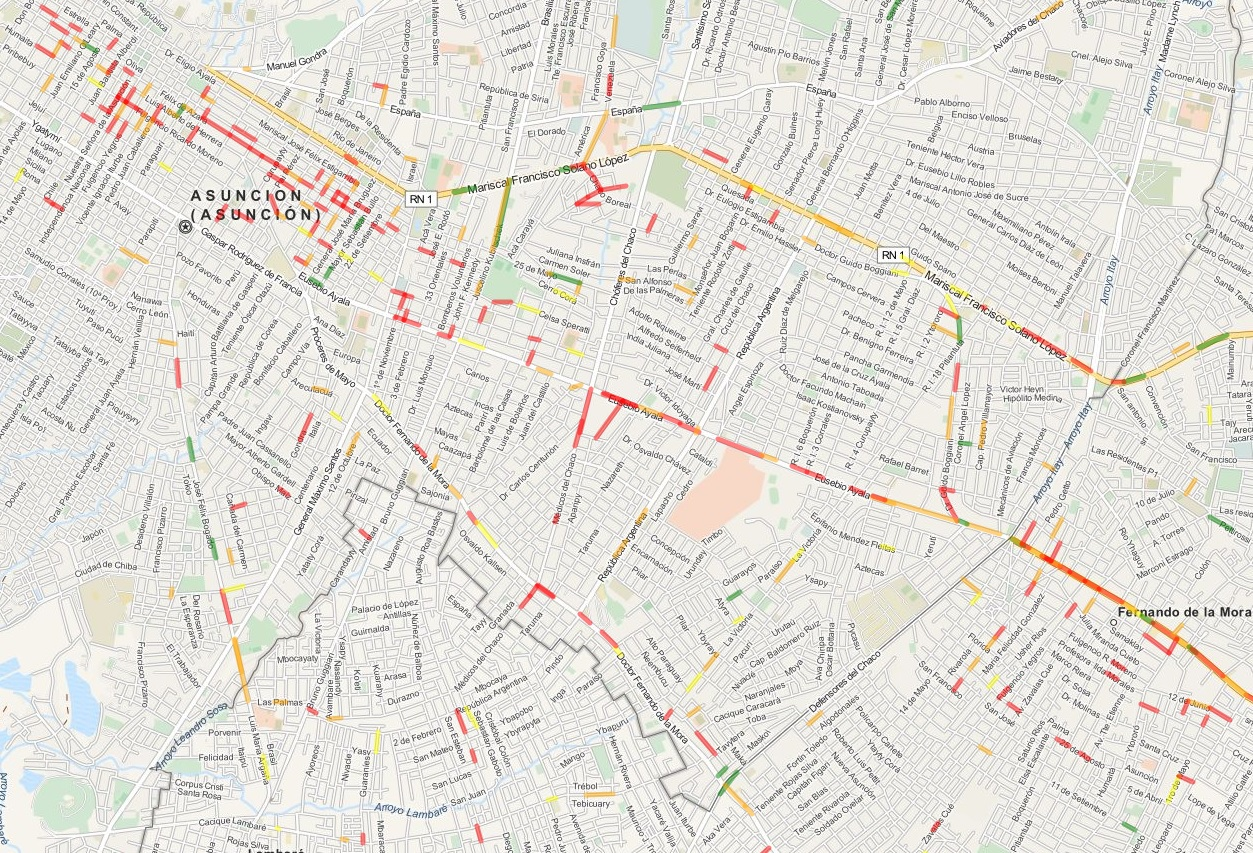
\includegraphics[width=0.7\textwidth]{capitulos/6/figuras/figura3.jpg}
	\caption{\label{fig:calles} Estado de calles en Autotracks}	
\end{figure}
